\documentclass[a4paper,BCOR7mm,12pt,pointlessnumbers,bibtotoc]{scrartcl}
% Define German as thesis language
%\usepackage{german}

\usepackage{latexsym,alltt,
            textcomp, float}

% Codierung
\usepackage[latin1]{inputenc}

% zusaetzliche Symbole
\usepackage{textcomp, latexsym}

% Grafiken
\usepackage{graphicx, psfrag}

% "H"-Option für Gleitumgebungen
\usepackage{float}

% Gleitumgebungen nach Referenz platzieren
\usepackage{flafter}

% lange Tabellen
\usepackage{longtable}

%Mathematik
\usepackage{amsmath}
\usepackage{amsfonts}
\usepackage{amssymb}

% pdftex
\usepackage{hyperref}

% neue deutsche Rechtschreibung
%\usepackage{ngerman}

% zusätzliche Spaltendefinitionen für Tabellen
\usepackage{array}

% Darstellung mehrerer Bilder als ein Objekt
\usepackage{subfigure}

% Drehen von Grafiken (turn,rotate)
\usepackage{rotating}
 
% Weitere Symbole
%\usepackage{psnfss}
\usepackage{pifont}

%Farben
\usepackage{color}

% Absatzabstand etwas groesser
\addtolength{\parskip}{1.1ex}

% Blocksatz erzwingen
\sloppy

% Abstand zweier Listenelemente kleiner
\setlength{\itemsep}{0ex plus0.2ex}

% "Rahmenabstand" für gerahmte Gleichungen
\setlength{\fboxsep}{10pt}

\begin{document}
%\maketitle
\begin{center}
\Large Hilbert Transformator IP Cores\\[0.4cm]
\large Martin Kumm \\[0.5cm]
\large \today \\[0.5cm]
\end{center}

\section{Introduction}

The Hilbert Transform is an important component in communication systems, e.g. for single sideband modulation/demodulation, amplitude and phase detection, etc. It can be formulated as filtering operation which makes it possible to approximate the Hilbert Transform with a digital filter. Due to the non-causal and infinite impulse response of that filter, it is not that easy to get a good approximation with low hardware resource usage. Therefore, different filters with different complexities have been implemented. The detailed discussion can be found in \cite{ks08}. 

\section{Mathematical Background}

The Hilbert Transform can be defined as filter in the discrete frequency domain as
\begin{equation}
H_{H}(e^{j \Omega}) =
 \left\{ 
    \begin{tabular}{ll}
    $-j$ & \mbox{for }\mbox{$0 < \Omega < \pi$}\\
    $j$ & \mbox{for }\mbox{$-\pi < \Omega < 0$}\\
    $0$ & \mbox{for }\mbox{$\Omega = 0$} \ \ ,\\
    \end{tabular}
 \right.
\end{equation}
with $\Omega=2\pi f/fs$, $f_s$ is the sampling frequency in Hz and $j=\sqrt{-1}$.
The magnitude is unity for all frequencies not equal to zero and the phase is $-90^\circ$ for all positive, and $+90^\circ$ for all negative frequencies. The inverse Fourier transform leads to the impulse response
\begin{equation}
h_{H}(n) = \frac{1-\cos(\pi n)}{\pi n} =
 \left\{ 
    \begin{tabular}{ll}
    $2/(\pi n)$ & \mbox{for }\mbox{odd}\mbox{ $n$}\\
    $0$ & \mbox{for }\mbox{even}\mbox{ $n$}.\\
    \end{tabular}
 \right.
 \label{equ:disc_hilbert_imp_resp}
\end{equation}
A so-called analytic signal can be generated from a real valued signal by extending the signal with its own Hilbert transform as the imaginary part:
\begin{equation}
	\underline{x}(n)=x(n)+j\mathcal{H}\{x(n)\}
	\label{equ:del_analytic_signal}
\end{equation}
This signal has the property that no spectral components exist for the lower half of the z-plane ($-\pi<\Omega<0$). The operation in (\ref{equ:del_analytic_signal}) can be formulated as a filter operation with
\begin{equation}
	\underline{H}_{A}(e^{j \Omega})=1+j H_{H}(e^{j \Omega}) \ \ .
	\label{equ:def_analytic_filter}
\end{equation}
The realizations are filters that generates an analytic signal from a real valued signal, therefore these filters are called analytic filter ($\underline{H}_{Ax}$). The implementations described in the next section realize analythic filters.

\section{Implementation}

The first analytic filter is implemented as FIR filter 
\begin{equation}
	\widetilde{H}_{H1}(z) = z^{-N/2} \sum_{k=-N/2}^{N/2} b_k z^{-k}
\end{equation}
Matlab (\verb|firls()|) was used to calculate the impulse response for an Hilbert filter with an order of $N=10$ to be $b_1=$163/256, $b_3=$54/256, $b_5=$32/256 and zero for all even coefficients. An additional delay is needed to form the analytic filter
\begin{equation}	
	\underline{H}_{A1}(z) = z^{-5} + j \widetilde{H}_{H1}(z) \ \ .
\end{equation}
Due to the zero coefficients and the asymmetric impulse response, only three real multipliers are needed. The structure of the implementation is shown in Figure~\ref{fig:h_a_1_filter_impl}. Two pipeline registers are implemented after the multiplication and the addition in the last stage. Therefore, the delay of the real part must be set to $z^{-7}$. Detailed plots of the filter are shown in Figure~\ref{fig:h_a1}.

\begin{figure}[H]
  \centering
    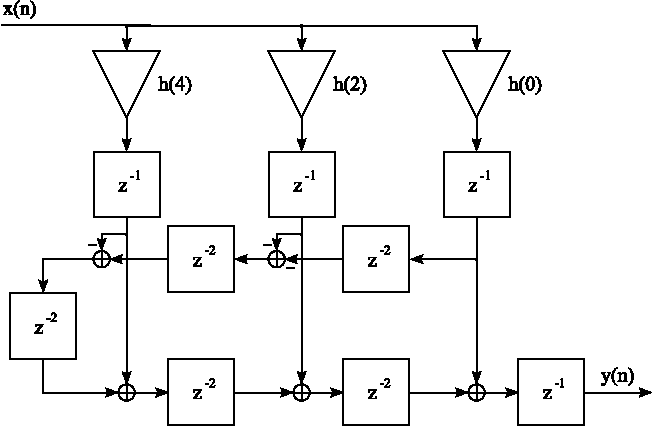
\includegraphics{images/h_a_1_filter_impl}
  \caption{Structure of $\widetilde{H}_{H1}(z)$}
  \label{fig:h_a_1_filter_impl}
\end{figure}

The following analytic filters are based on frequency sampling filters (see \cite{ks08} for further details), so only the transfer functions are given here:
\begin{equation}
  \underline{H}_{A2}(z) = F_{z4}(z)C_{+90}(z)
\end{equation}
with
\begin{equation}	
  F_{z4}(z) = 1-z^{-4}
\end{equation}
and
\begin{equation}	
  C_{+90}(z) = \frac{z^{-1}}{1 - j z^{-1}} \ \ .
\end{equation}
Detailed plots of the filter are shown in Figure~\ref{fig:h_a2}. 

The third one is defined as 
\begin{equation}	
  \underline{H}_{A3}(z) = \left(\underline{H}_{A2}(z)C_{0/180}(z)C^{-1}_{-30/-150}(z)\right)^{2}
\end{equation}
with
\begin{equation}	
  C_{0/180}(z) = \frac{z^{-2}}{1 - z^{-2}}
\end{equation}
and
\begin{equation}	
  C^{-1}_{-30/-150}(z) = (1 + j z^{-1} - z^{-2}) \ \ .
\end{equation}
Detailed plots of the filter are shown in Figure~\ref{fig:h_a3}. A block diagram of the implementation is shown in Figure~\ref{fig:block_impl_h_a3}.

\begin{figure}[H]
  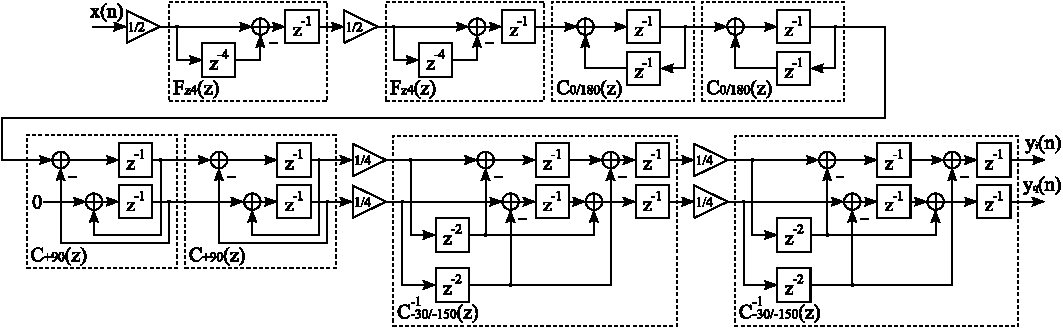
\includegraphics[width=15 cm]{images/block_impl_h_a3}
  \caption{Block diagram of  $\underline{H}_{A3}(z)$}
  \label{fig:block_impl_h_a3}
\end{figure}

The last filter is an extension of $\underline{H}_{A3}(z)$ with an IIR component, so the total impulse response becomes IIR ($\underline{H}_{A1-A3}(z)$ have a finite impulste response even though IIR components are included). The transfer function is
\begin{equation}
  \underline{H}_{A4}(z) = \underline{H}_{A3}(z) C_{P}^2(z)
\label{equ:fsf_ha4_cp}
\end{equation}
with
\begin{equation}	
  C_{P}(z) = \frac{z^{-2}}{1-\frac{1}{2} z^{-2}} \ \ .
\label{equ:cp}
\end{equation}

Detailed plots of the filter are shown in Figure~\ref{fig:h_a4}. A block diagram of the implementation is shown in Figure~\ref{fig:block_impl_h_a4}.

\begin{figure}[H]
	\includegraphics[width=15 cm]{images/block_impl_h_a4}
	\caption{Block diagram of  $\underline{H}_{A4}(z)$}
	\label{fig:block_impl_h_a4}
\end{figure}

\section{Comparison of the Filters}

The resource usage of the filters is shown in Table~\ref{tab:filter_performance}. All filters have been compiled for an Altera Cyclone I FPGA (EP1C6Q240C8).

\begin{table}[H]
  \centering
    \begin{tabular}{l|r|r|r|r}
      \hline
      \hline
        Filter         & $N_A$ & $N_R$ & $N_{LE}$ & $f_{max}$ [MHz]\\
        \hline                        
        $\underline{H}_{A1}(z)$ & 10    & 6  & 337 & 266\\
        $\underline{H}_{A2}(z)$ & 3     & 4  & 110 & 275\\ 
        $\underline{H}_{A3}(z)$ & 16    & 18 & 562 & 191\\
        $\underline{H}_{A4}(z)$ & 18    & 38 & 679 & 193\\ 
      \hline
      \hline
    \end{tabular}
  \caption{Ressource usage of the implemented filters. Symbols: $N_A$, $N_R$ and $N_{LE}$: required number of adders/subtracters (incl. output register), registers (incl. pipeline registers) and logic elements on Altera Cyclone I, $f_{max}$: maximum speed on Altera Cyclone I. The constant coefficient multipliers of $\underline{H}_{A1}(z)$ were represented by equivalent adders using the canonic signed digit system \cite{mb07} for comparison.}
  \label{tab:filter_performance}
\end{table}

\section{Frequency Responses of the implemented Filters}

\begin{figure}[H]
  \centering
  \subfigure[]{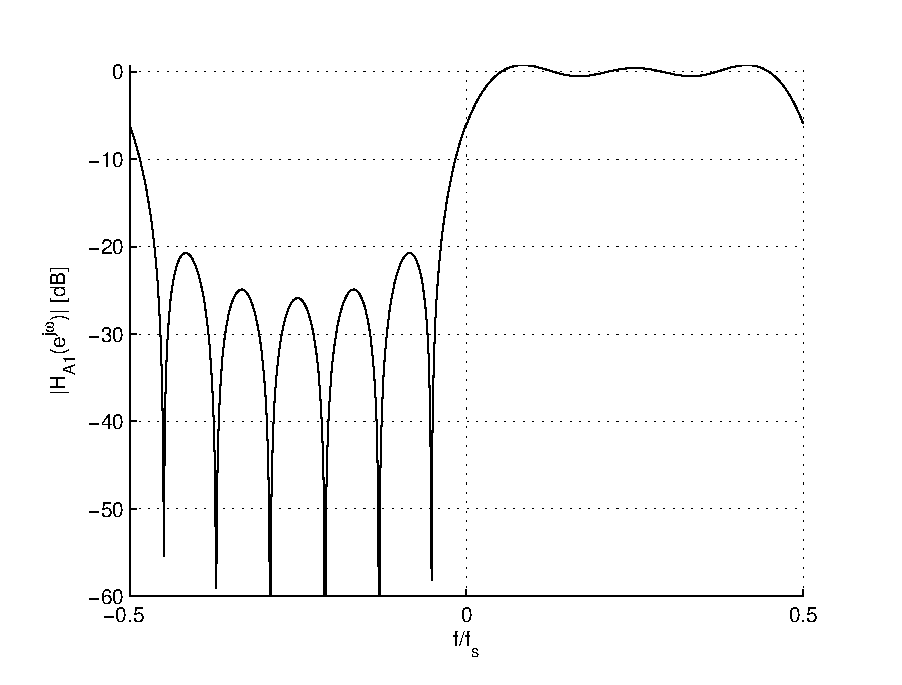
\includegraphics[width=65 mm]{images/h_a1_total_abs}\label{fig:h_a1_total_abs}}
  \subfigure[]{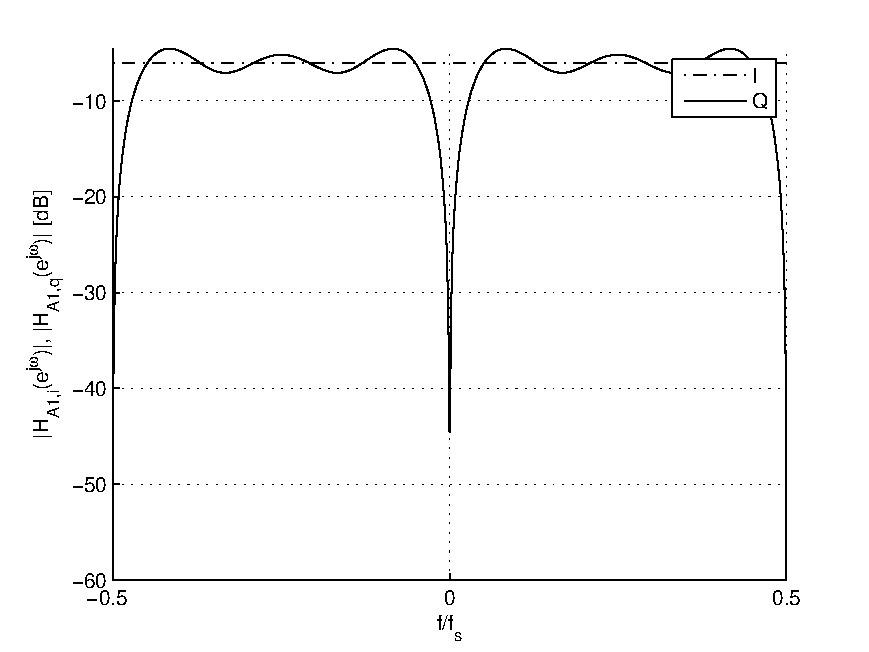
\includegraphics[width=65 mm]{images/h_a1_iq_abs}\label{fig:h_a1_iq_abs}}
  \subfigure[]{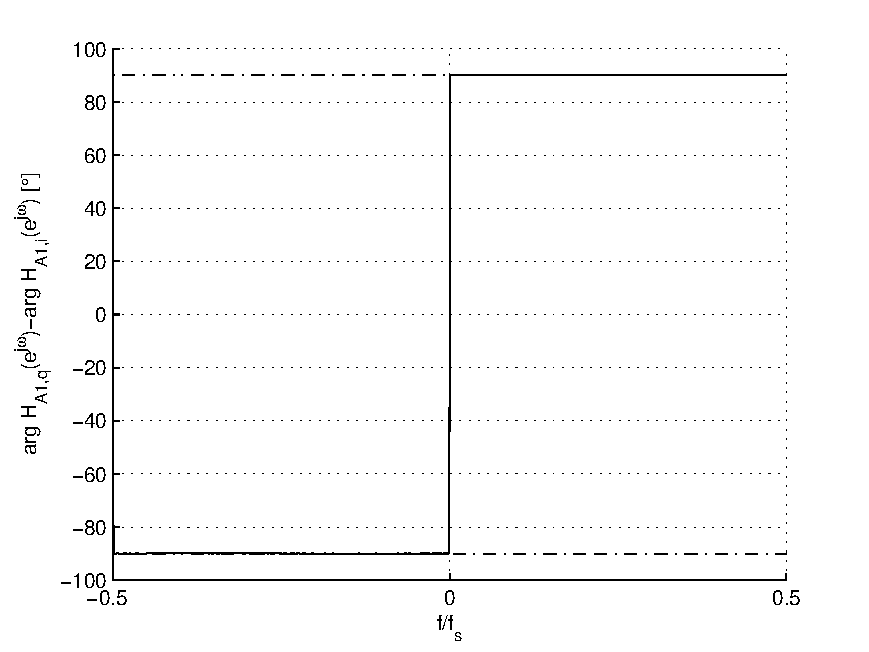
\includegraphics[width=65 mm]{images/h_a1_phase_diff}\label{fig:h_a1_phase_diff}}
  \subfigure[]{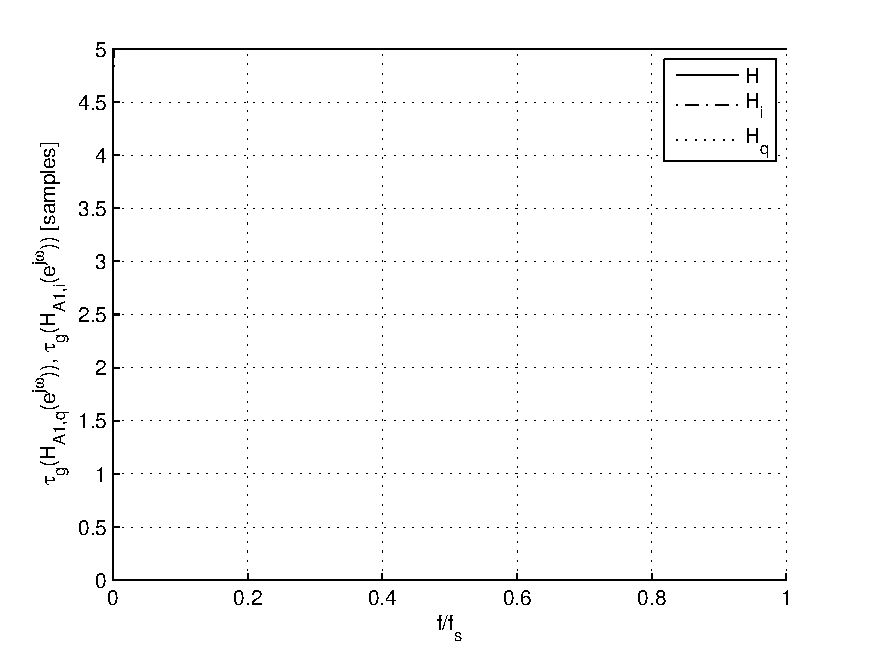
\includegraphics[width=65 mm]{images/h_a1_iq_gd}\label{fig:h_a1_iq_gd}}
  \subfigure[]{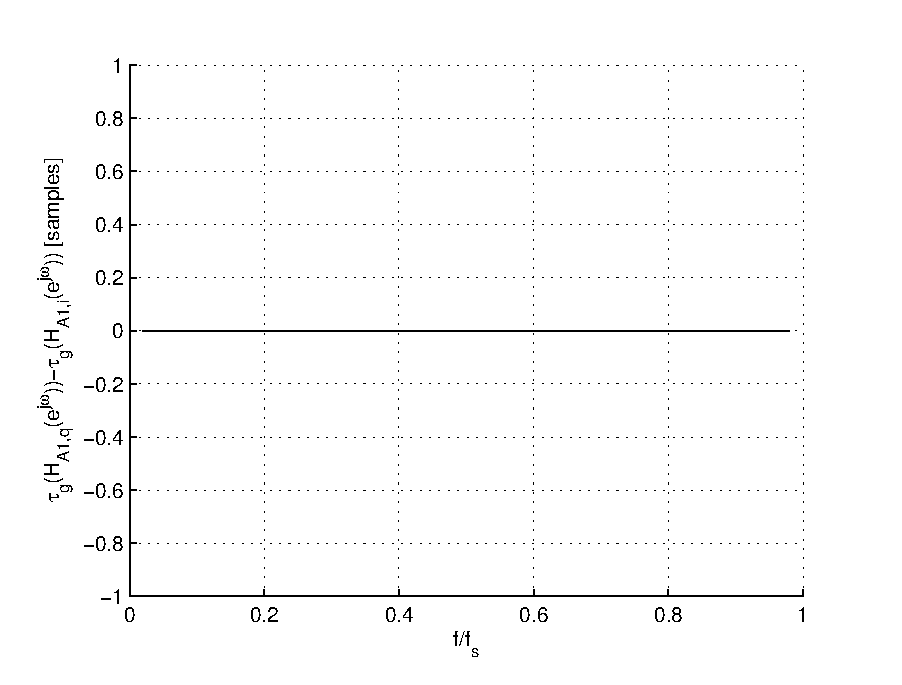
\includegraphics[width=65 mm]{images/h_a1_iq_diff}\label{fig:h_a1_iq_diff}}
  \subfigure[]{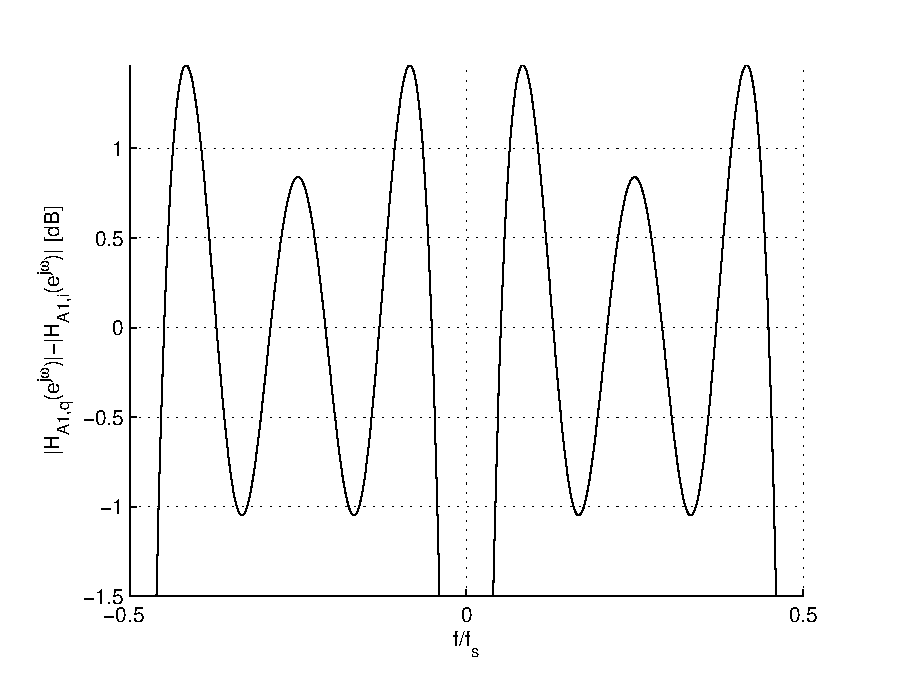
\includegraphics[width=65 mm]{images/h_a1_iq_ampl_mismatch}\label{fig:h_a1_iq_ampl_mismatch}}
  \caption{Plots of the filter $H_{A1}(e^{j \omega})$, (a) normalized magnitude response of the total filter, (b) normalized magnitude response of the real and imaginary parts (I and Q), (c) phase response, (d) group delay of the total filter and I and Q paths, (e) group delay error between I and Q, (f) amplitude error between I and Q}
  \label{fig:h_a1}
\end{figure}

\begin{figure}[H]
	\centering
  \subfigure[]{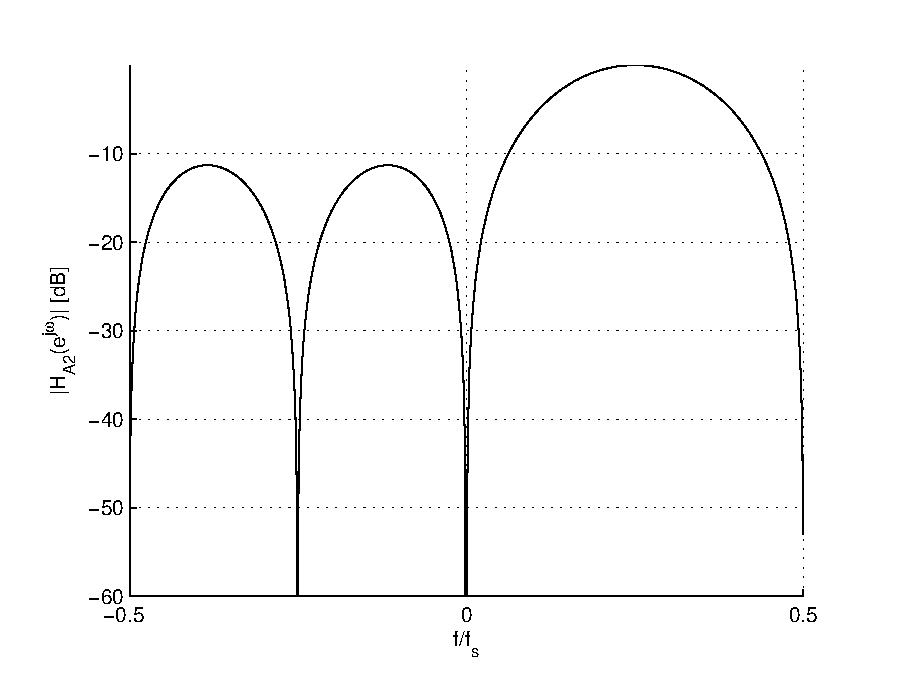
\includegraphics[width=65 mm]{images/h_a2_total_abs}\label{fig:h_a2_total_abs}}
  \subfigure[]{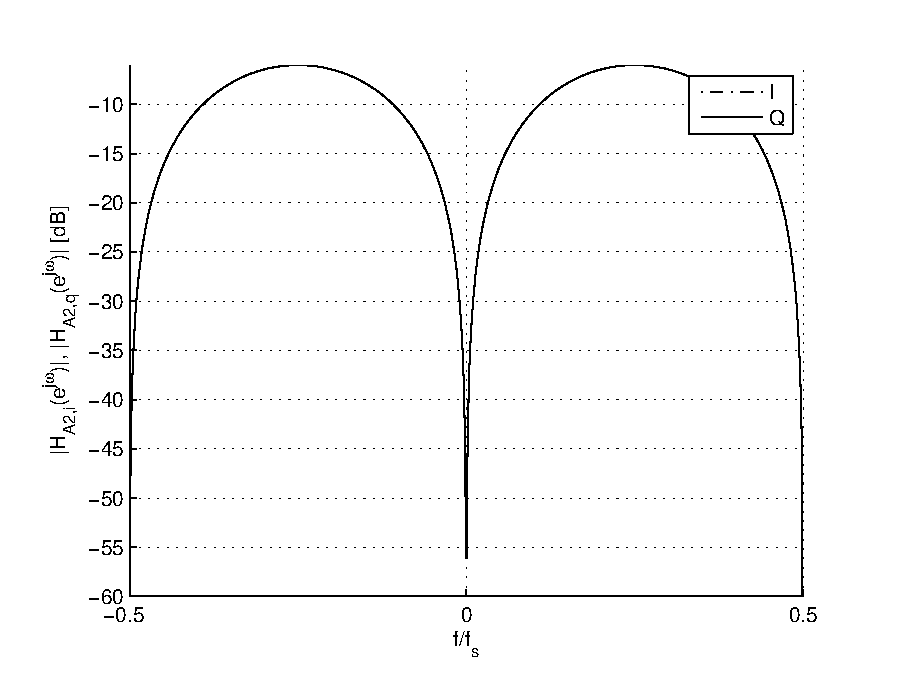
\includegraphics[width=65 mm]{images/h_a2_iq_abs}\label{fig:h_a2_iq_abs}}
  \subfigure[]{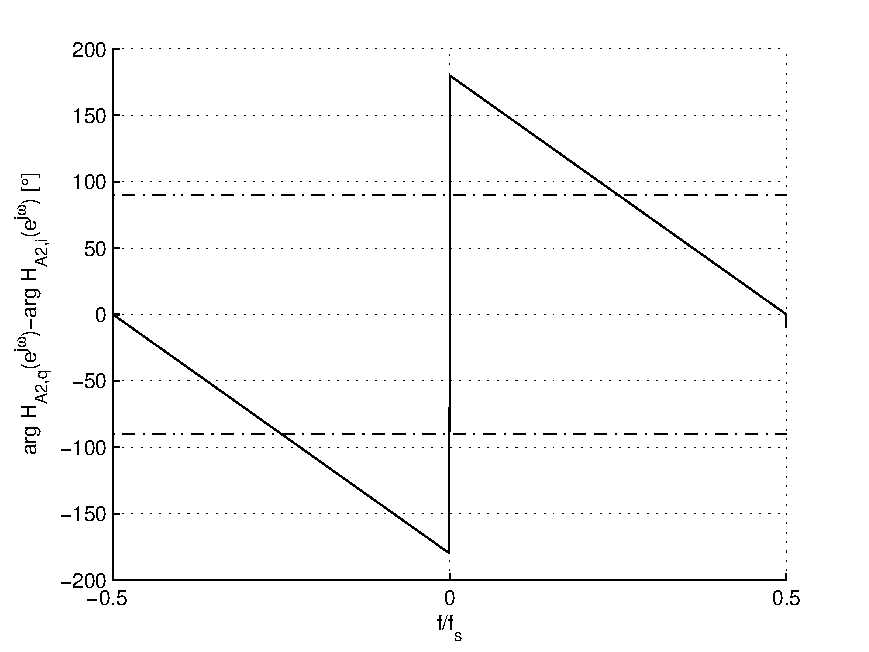
\includegraphics[width=65 mm]{images/h_a2_phase_diff}\label{fig:h_a2_phase_diff}}
  \subfigure[]{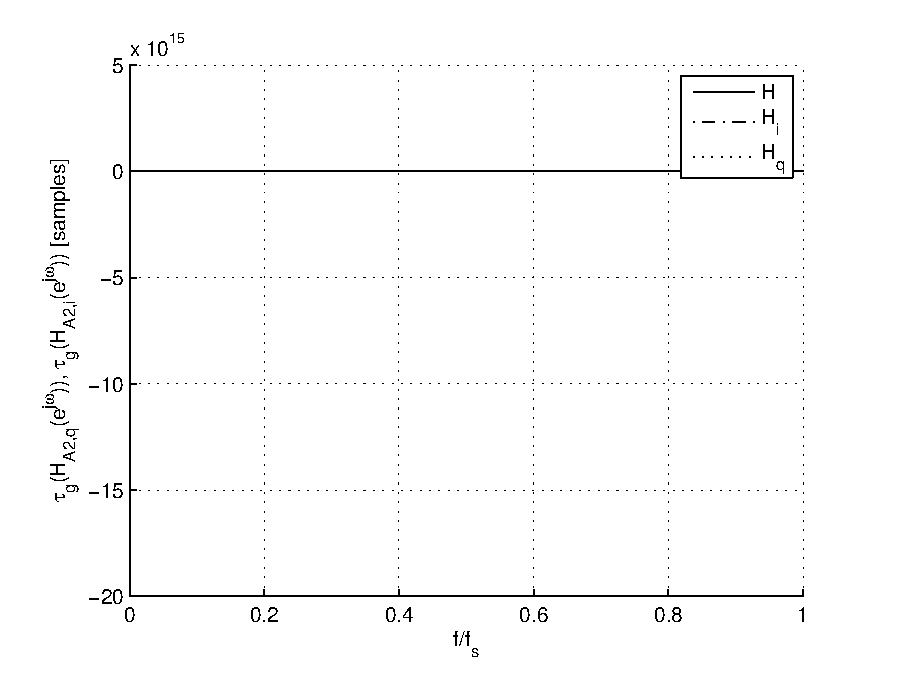
\includegraphics[width=65 mm]{images/h_a2_iq_gd}\label{fig:h_a2_iq_gd}}
  \subfigure[]{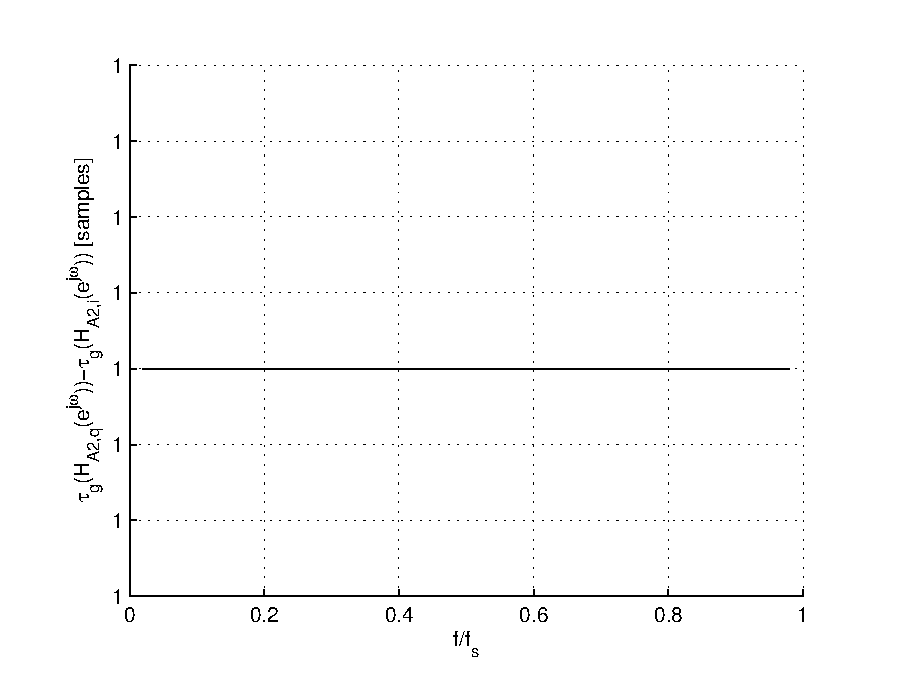
\includegraphics[width=65 mm]{images/h_a2_iq_diff}\label{fig:h_a2_iq_diff}}
  \subfigure[]{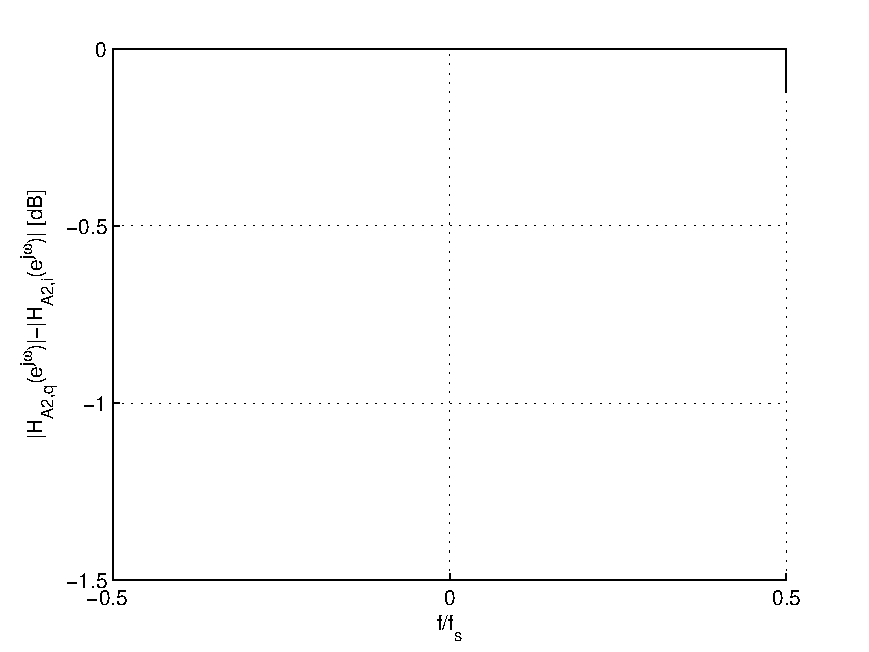
\includegraphics[width=65 mm]{images/h_a2_iq_ampl_mismatch}\label{fig:h_a2_iq_ampl_mismatch}}
  \caption{Plots of the filter $H_{A2}(e^{j \omega})$, (a) normalized magnitude response of the total filter, (b) normalized magnitude response of the real and imaginary parts (I and Q), (c) phase response, (d) group delay of the total filter and I and Q paths, (e) group delay error between I and Q, (f) amplitude error between I and Q}
  \label{fig:h_a2}
\end{figure}

\begin{figure}[H]
	\centering
  \subfigure[]{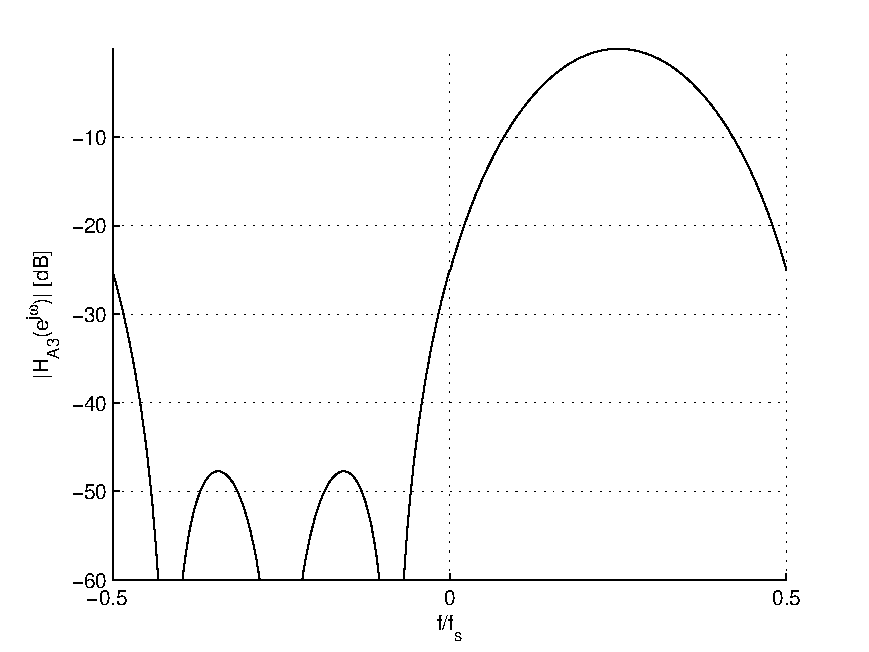
\includegraphics[width=65 mm]{images/h_a3_total_abs}\label{fig:h_a3_total_abs}}
  \subfigure[]{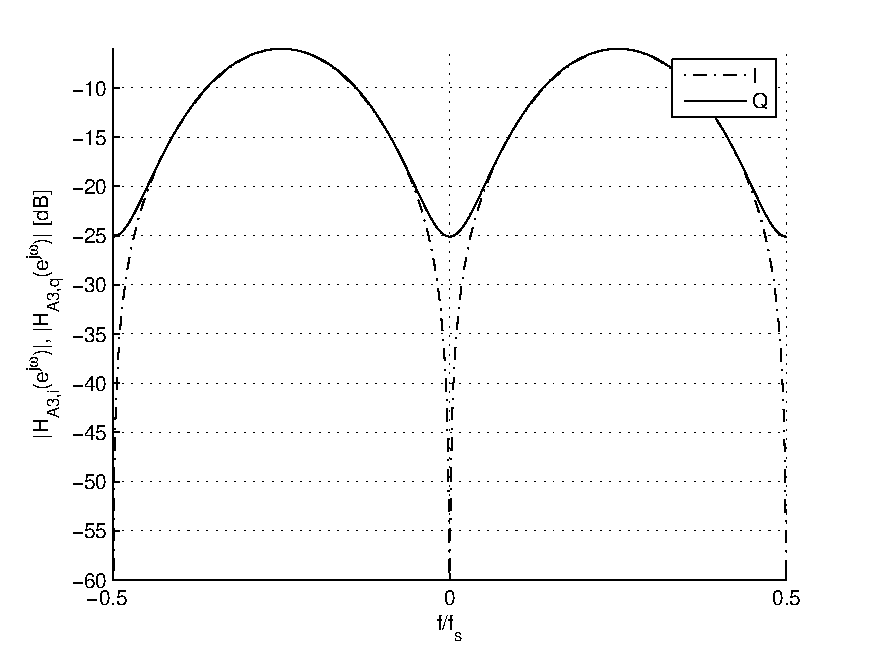
\includegraphics[width=65 mm]{images/h_a3_iq_abs}\label{fig:h_a3_iq_abs}}
  \subfigure[]{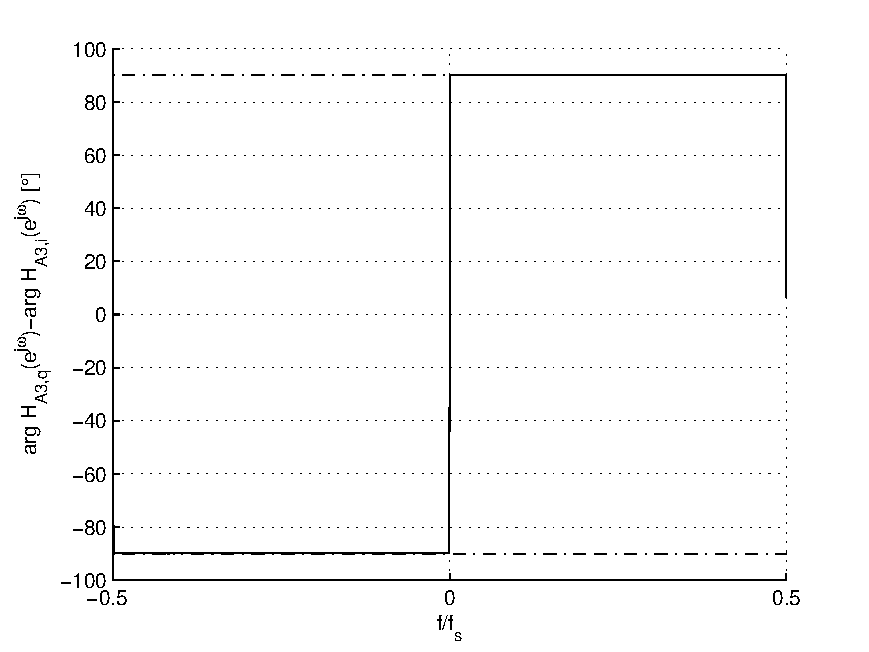
\includegraphics[width=65 mm]{images/h_a3_phase_diff}\label{fig:h_a3_phase_diff}}
  \subfigure[]{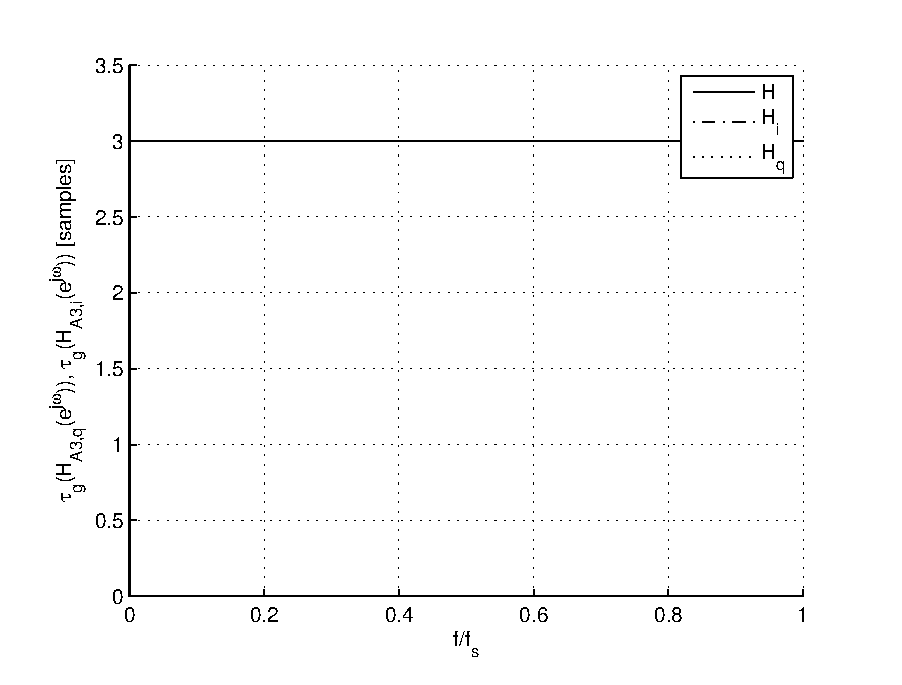
\includegraphics[width=65 mm]{images/h_a3_iq_gd}\label{fig:h_a3_iq_gd}}
  \subfigure[]{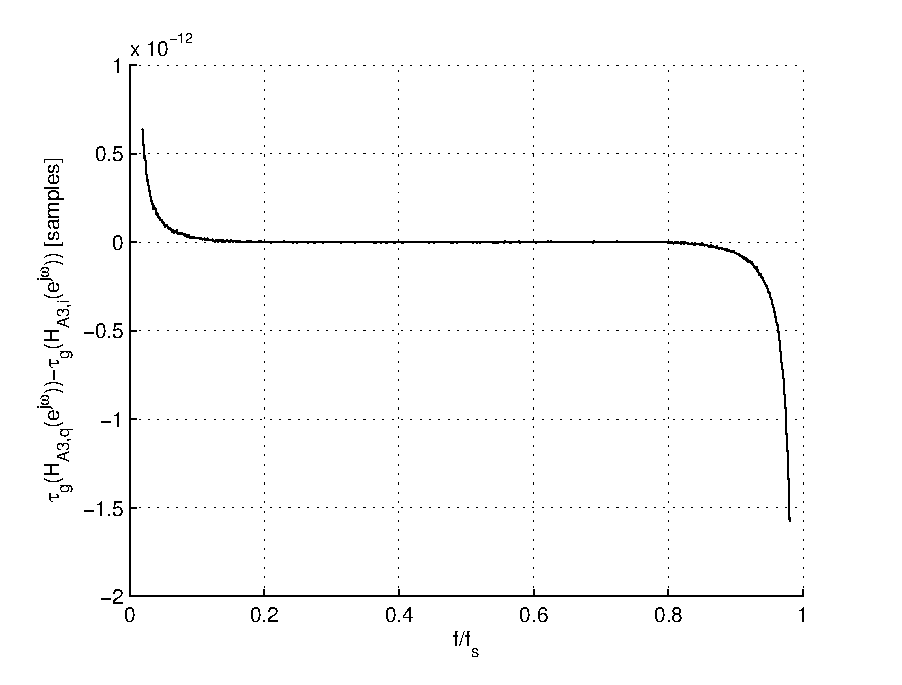
\includegraphics[width=65 mm]{images/h_a3_iq_diff}\label{fig:h_a3_iq_diff}}
  \subfigure[]{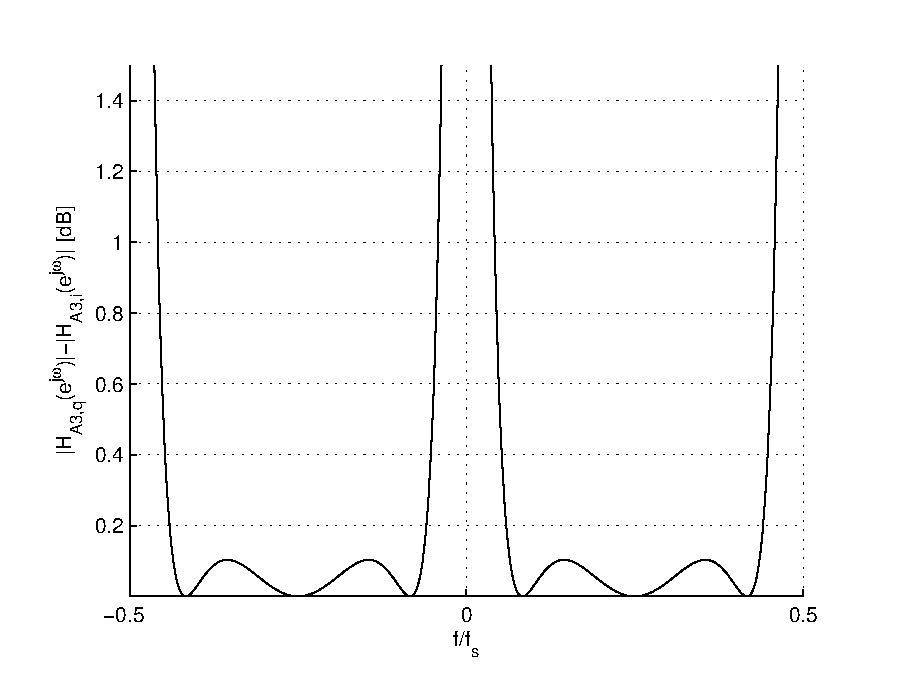
\includegraphics[width=65 mm]{images/h_a3_iq_ampl_mismatch}\label{fig:h_a3_iq_ampl_mismatch}}
  \caption{Plots of the filter $H_{A3}(e^{j \omega})$, (a) normalized magnitude response of the total filter, (b) normalized magnitude response of the real and imaginary parts (I and Q), (c) phase response, (d) group delay of the total filter and I and Q paths, (e) group delay error between I and Q, (f) amplitude error between I and Q}
	\label{fig:h_a3}
\end{figure}

\begin{figure}[H]
	\centering
  \subfigure[]{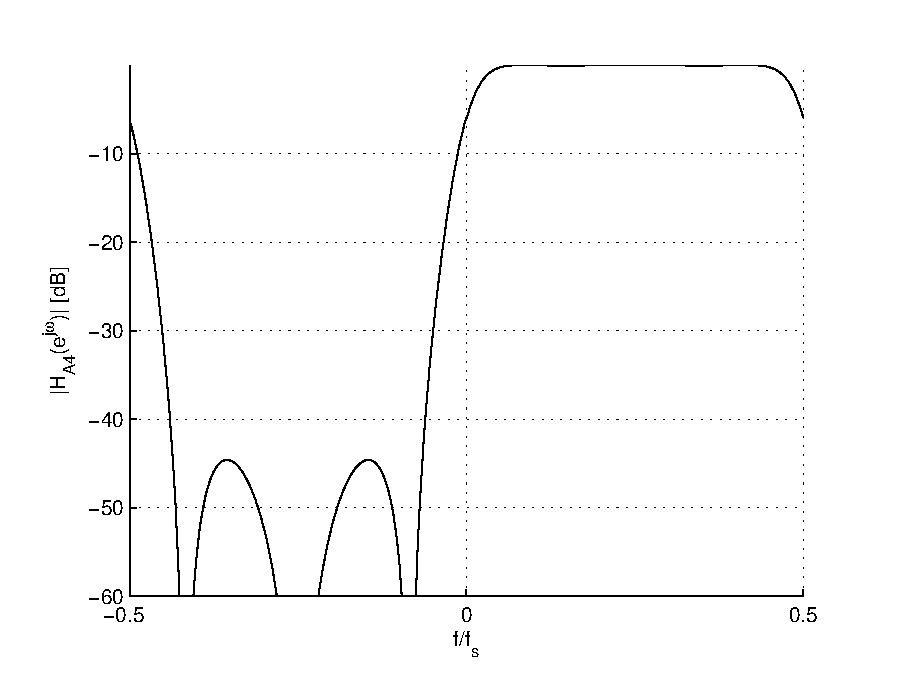
\includegraphics[width=65 mm]{images/h_a4_total_abs}\label{fig:h_a4_total_abs}}
  \subfigure[]{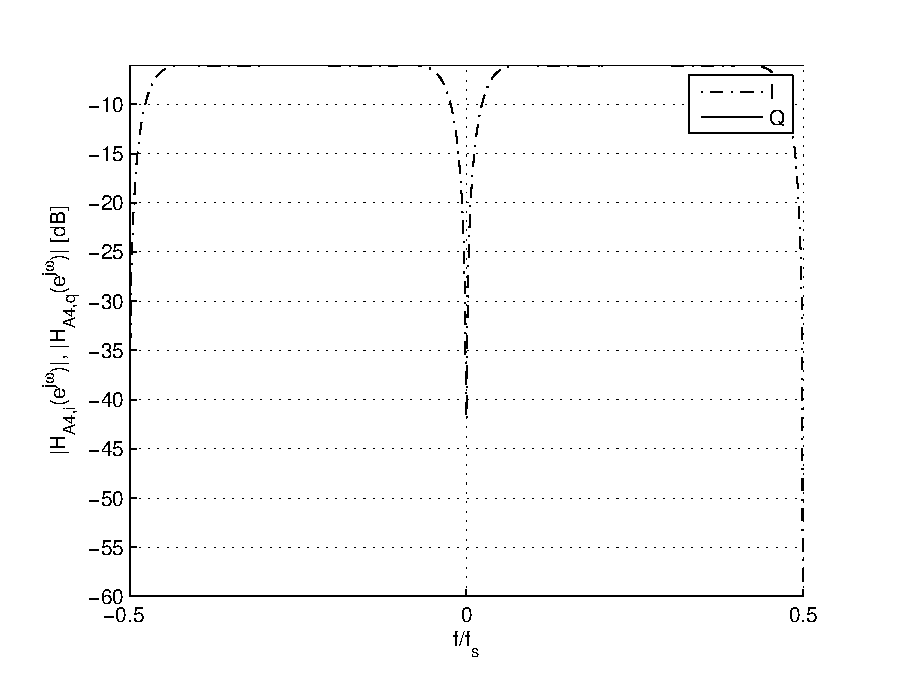
\includegraphics[width=65 mm]{images/h_a4_iq_abs}\label{fig:h_a4_iq_abs}}
  \subfigure[]{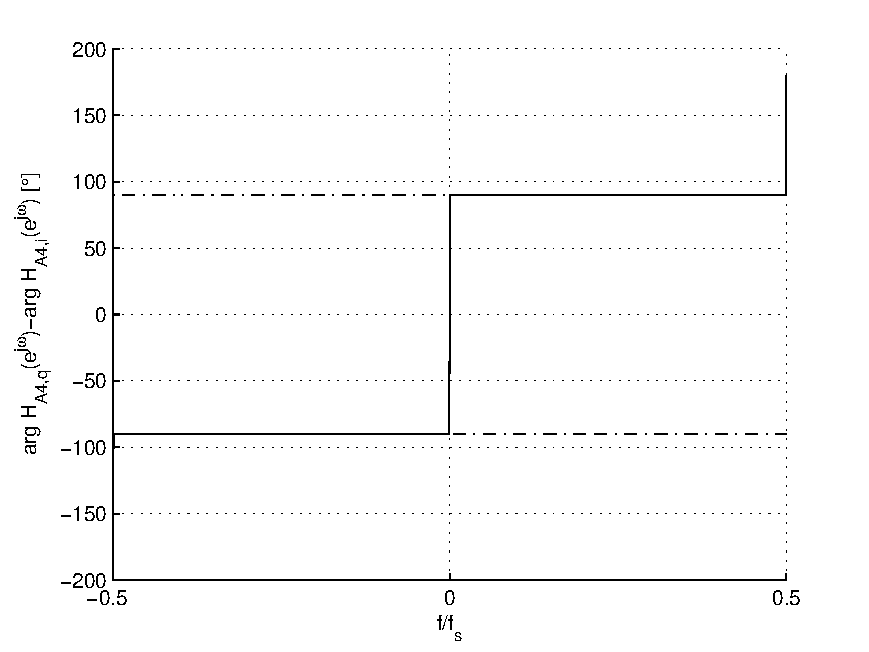
\includegraphics[width=65 mm]{images/h_a4_phase_diff}\label{fig:h_a4_phase_diff}}
  \subfigure[]{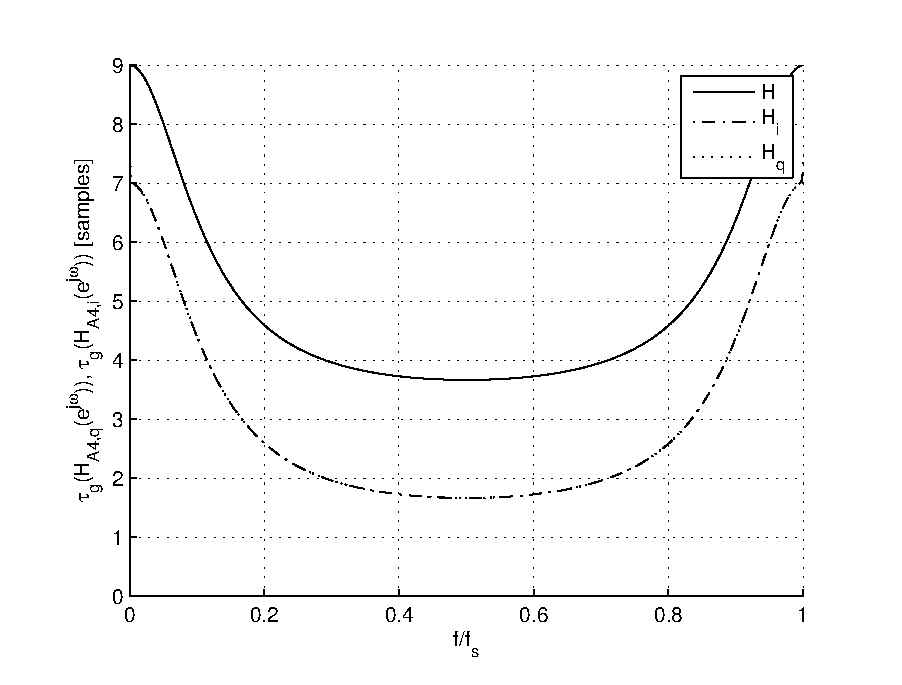
\includegraphics[width=65 mm]{images/h_a4_iq_gd}\label{fig:h_a4_iq_gd}}
  \subfigure[]{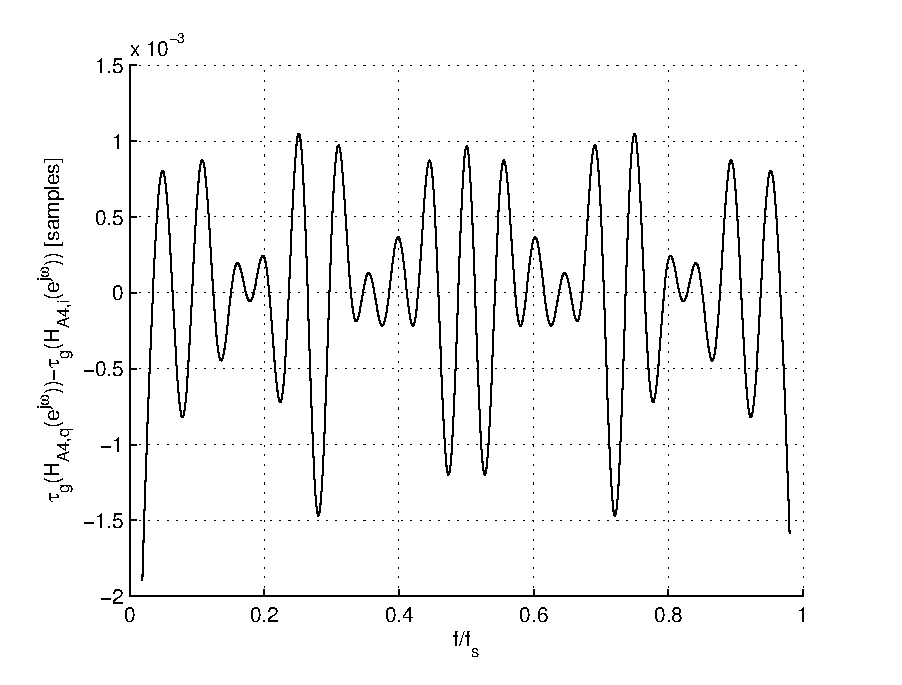
\includegraphics[width=65 mm]{images/h_a4_iq_diff}\label{fig:h_a4_iq_diff}}
  \subfigure[]{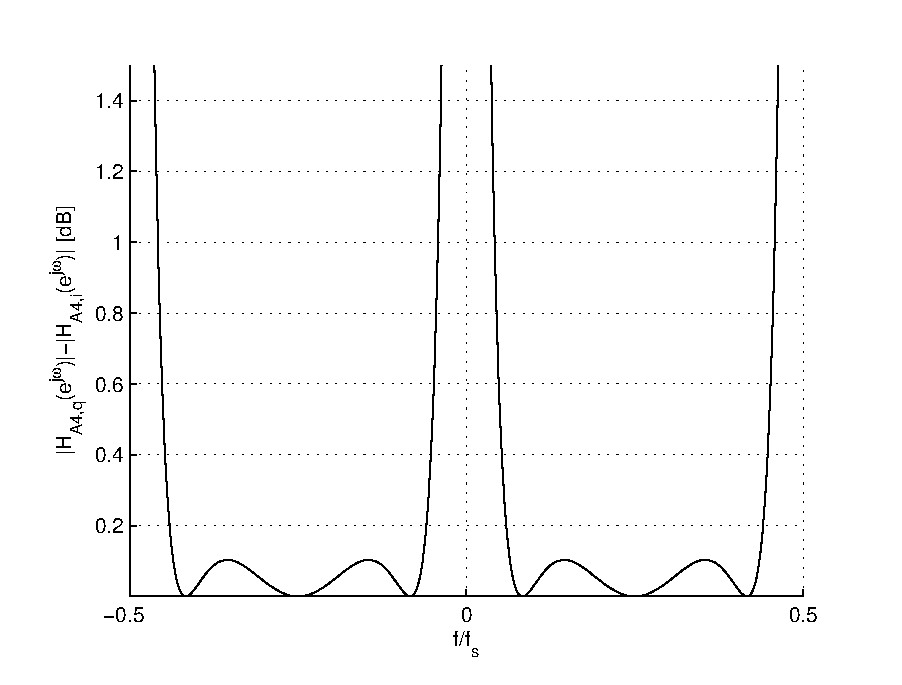
\includegraphics[width=65 mm]{images/h_a4_iq_ampl_mismatch}\label{fig:h_a4_iq_ampl_mismatch}}
  \caption{Plots of the filter $H_{A4}(e^{j \omega})$, (a) normalized magnitude response of the total filter, (b) normalized magnitude response of the real and imaginary parts (I and Q), (c) phase response, (d) group delay of the total filter and I and Q paths, (e) group delay error between I and Q, (f) amplitude error between I and Q}
  \label{fig:h_a4}	
\end{figure}


\bibliographystyle{alpha}
\bibliography{hilbert_transformer}

\end{document}


 
